\documentclass[12pt,a4paper]{article}
\usepackage[english,german]{babel}
\usepackage[utf8]{inputenc}
\usepackage{color}
\usepackage{hyperref}
\usepackage{mathtools}
\usepackage{amsmath}
\usepackage{graphicx}
\usepackage{enumitem}

\usepackage{geometry}
\geometry{
  left=3cm,
  right=3cm,
  top=3cm,
  bottom=4cm,
  bindingoffset=5mm
}

\setlength{\parindent}{0em} 
\hypersetup{
    colorlinks=true,
    linktoc=all,
    linkcolor=black,
    urlcolor=black
}

% Hurenkinder und Schusterjungenregel
\clubpenalty = 10000
\widowpenalty = 10000
\displaywidowpenalty = 10000

%Gummi|065|=)
\title{Einsprechthema}
\author{}
\date{}

% set title of table of contents
\renewcommand*\contentsname{Inhalt}

% https://www.sharelatex.com/learn
% http://www.math.ubc.ca/~cautis/tools/latexmath.html
% http://www.golatex.de/wiki/Kategorie:Befehlsreferenz
% https://en.wikibooks.org/wiki/LaTeX/Mathematics

\begin{document}

\begin{titlepage}

\maketitle
\thispagestyle{empty}
\end{titlepage}
\newpage

\section{Aufbau Neuron}
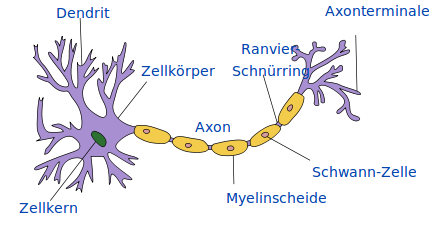
\includegraphics[width=0.6\textwidth]{tmp_pix/neuron.png}

\section{Arten}
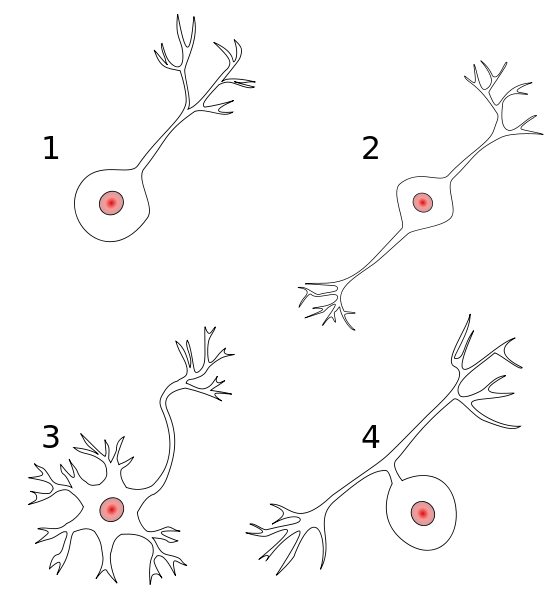
\includegraphics[width=0.5\textwidth]{tmp_pix/kinds_of_neuron.png}\\
1. unipolare Nervenzelle, 2. bipolare Nervenzelle, 3. multipolare Nervenzelle, 4. pseudounipolare Nervenzelle\\

\subsection{genauere Erklärung Axon}
\begin{enumerate}
	\item Axonhügel: pyramidenförmige Vorwölbung
	\item Initialsegement: anschließende kurze Segment des Fortsatzes und stets ohne Hülle
	\item Hauptverlaufsstrecke:
	\item Endverzweigung: präsynaptischen Teil einer Synapse
\end{enumerate}

Myelinscheide, Schwann-Zelle, Ranvier-Schnürring

\subsection{neuronale Wegfindung}
\begin{itemize}
	\item Wachstumskegel bilden ständig sehr bewegliche Filopodien (bis 50 $\mu$m), die auch wieder zurückgebildet werden können
	\item die Beweglichkeit beruht auf der Polymerisation und Depolymerisation von Actin-Mikrofilamenten, was mit einem Membran-Turn-over (Endo-Exocytose von Membranvesikeln) verbunden ist
\end{itemize}

\textbf{Chemoaffinitätstheorie:} Erkennung der Zielzellen durch chem. Markierung\\\\
4 Mechanismen der Wegfindung:
\begin{itemize}
	\item Klassische Chemotaxis = gerichtetes Wachstum nach Stoffgradienten: anziehend bzw. abstoßend
	\item Kontaktführung (contact guidance) = Präferenz für spezielle Substrate (selektive Ahhäsion): anziehend (Polyornithrin) bzw. abstoßend (Palladium)
\end{itemize}

\textbf{Wachstumsgeschwindigkeit:} bis 1mm / Tag

\section{Signale und Verarbeitung}

\subsection{EPSP und IPSP}
Ob ein NT erregend (exzitatorisch) oder hemmend (inhibitorisch) wirkt, hängt ausschließlich von der Art der postsynaptischen Rezeptormolekülen ab:
\begin{itemize}
	\item erregend: Bildung eines EPSPs (exzitatorisches postsynaptisches Potential)
	\item hemmend: Bildung eines IPSPs (inhibitorisches postsynaptisches
Potential)
\end{itemize}

\subsection{Summation zeitlich und räumlich}
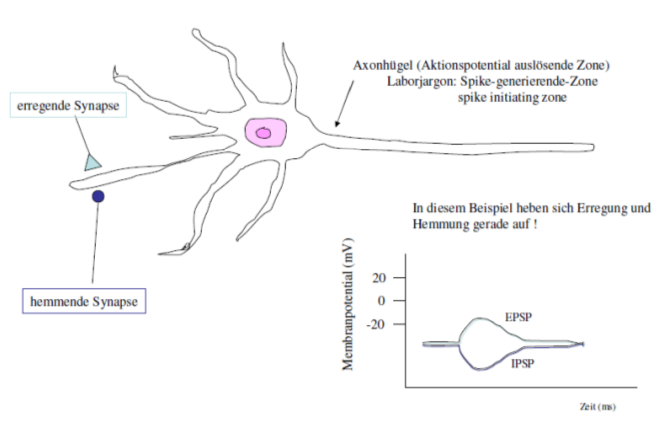
\includegraphics[width=0.6\textwidth]{tmp_pix/calculation.png}

\underline{räumliche Summation:} EPSPs/IPSPs verschiedener Synapsen, die z.B. an einem Dendritenbaum ansetzen, werden in der postsynaptischen Zelle zu jedem Zeitpunkt addiert\\

\underline{zeitliche Summation:} Die in einer Präsynapse zeitlich kurz aufeinanderfolgenden Aktionspotentiale lösen in der postsynaptischen Zeller EPSPs/IPSPs aus, welche addiert werden.
Für die Integration sind die passiven elektrischen Eigenschaften (Kabeleigenschaften) des postsynaptischen Neurons sehr wichtig.

%\subsection{Prinzipien der Verschaltung}

\section{Aktionspotential}
	\begin{itemize}
		\item Ausgangslage: Ruhemembranpotential (-70mV; gleichstarker Ein- und Ausstrom von K+)
		\item Initiationsphase: Zunahme des Potentials bis mind. Schwellwert (-50mV) (vorher nur unterschellige Reize)
		\item Depolarisierung: Einströmen von Na+
		\item Overshot: bei ca. -60mV beginnen Na+-Kanäle sich zu öffenen, wodurch sehr viel Natrium in sehr kurzer Zeit einstömen kann $\rightarrow$ OVERSHOT (Membranpotential positiv, ca. 30mV)
		\item Repolarisierung: nach der maximalen Öffnung der Natriumkanäle werden diese wieder geschlossen, zusätzlich verzögerter K+ Ausstrom $\rightarrow$ Potential sinkt, Rückkehr zur Ausgangslage
		\item Hyperpolarisierung: durch eine noch anhaltende erhöhte Kaliumleitfähigkeit kommt es zum unterschreiten der Ausgangslage (bis ca. 90mV) $\rightarrow$ Gleichgewicht der Leitfähigkeiten stellt sich dann ein $\rightarrow$ entgültige Rückkehr zum Ruhemembranpotential (-70mV), Dauer des Aktionspotentials ca. 2ms
		\item Refraktärzeit: Na+-Kanäle brauchen Zeit für eine Wiederaktivierung $\rightarrow$ kein sofortiges Reizen möglich; kurz nach dem Overshot Schwellwert "unendlich" -> absolute Refraktärzeit von ca. 0,5ms; danach folgt relative Refraktärzeit von ca.3,5ms $\rightarrow$ hier Reizung durch erhöhtes Aktionspotential möglich
	\end{itemize}

\section{Zusätzlich werden Ca2+-Kanäle geöffnet}
Vesikel können Neurotransmitter an synaptischen Spalt freigeben\\\\
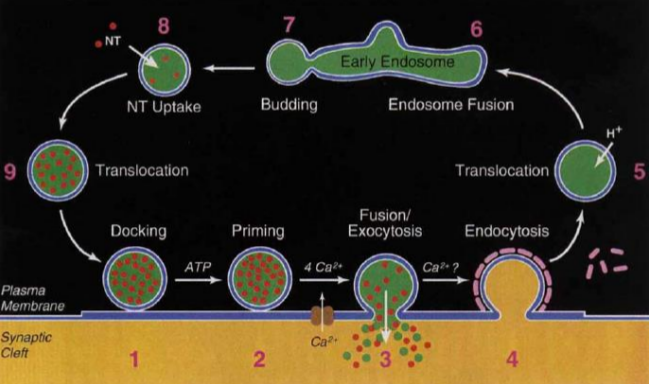
\includegraphics[width=0.6\textwidth]{tmp_pix/vesikel.png}

\textbf{Kreislauf in 9 Schritten:}
\begin{enumerate}
	\item Docking an Membran
	\item Priming: Vorbereitung für Exozytose (Verbrauch von ATP)
	\item Fusion/Exozytose: bei Aufnahme von Ca$^{2+}$ über kalziumabhängigen Ionenkanal wird die Exozytose eingeleitet und die Neurotransmitter werden in den synaptischen Spalt abgegeben
	\item Endozytose
	\item Translocation: H$^+$-Ionen werden in Visikel aufgenommen und reservieren Platz für neue Neurotransmitter
	\item endosome Fusion: Visikel geht in Reservepool über
	\item Budding: Abspaltung eines neuen Visikels
	\item NT uptake: Aufnahe von Neurotransmittern
	\item Translokation: Bewegung innerhalb der Synapse (Plasma) in Richtung Membran
\end{enumerate}

\textbf{SNARE-Proteinkomplexe und Toxine}\\
spalten SNARE-Proteine, wodurch die Vesikelfusion und somit die
Transmitterfreisetzung verhindert wird
\begin{itemize}
	\item Botulinum Toxine $\rightarrow$ Fleischvergiftung, Tod durch Lähmung der Atmung
	\item Tetanus Toxin
\end{itemize}

\section{Welche Neurotransmitter gibt es?}
\textbf{\underline{Acetylcholin}}\footnote{\url{https://de.wikipedia.org/wiki/Acetylcholin}} als wichtigster Neurotransmitter\\\\
weitere:
\begin{itemize}
	\item biogene Amine: Adrenalin, Serotonin
	\item Aminosäuren: GABA (Gamma-Amino-Butteracid), Glycin, Glutamat
	\item Peptide: Opioide, Substanz P, Insulin
	\item gasförmige Transmitter: Stickoxid, Kohlenmonoxid
\end{itemize}

\underline{zu Substanz P:}
\begin{itemize}
	\item Neurotransmitter bei Schmerzrezeptoren, stärkere Erregung $\rightarrow$ setzt Substanz P frei, spielt auch als Modulator bei Entzündungen eine Rolle
	\item Capsaicin $\rightarrow$ aktiviert die Hitzerezeptoren in der Mundschleimhaut $\rightarrow$ Ausschüttung von Substanz P ins Gewebe $\rightarrow$ schmerzartigen Empfindungen, bei regelmäßiger Verwendung von Capsaicin gewöhnt sich der Körper daran und die Menge an ausgeschütteter Substanz P wird geringer.
	\item Innerhalb der Säugetiere fehlt Substanz P beim Nacktmull, der damit vermutlich eine gewisse Schmerzresistenz aufweist.
\end{itemize}

\textcolor{red}{\textbf{$\Rightarrow$ erste Wandlung: AD $\rightarrow$ von kontinuierlichem Signal (Potential) zu diskretem Signal (Anzahl Neurotransmitter)}}

\section{NTs strömen in Richtung Postsynapse, Aufnahme der Neurotransmitter über Rezeptormoleküle:}
	\begin{enumerate}
		\item Ionotrope Rezeptoren (ATPasen, Ionenkanäle) $\rightarrow$ führt zur Änderung des Membranpotentials
		\item Metabotrope Rezeptoren: Ionenstrom wird indirekt vermittel $\rightarrow$ G-Protein-gekoppelte Rezeptoren (second messenger Prinzip erklären) $\rightarrow$ führt zu einem An- und Ausschalten (Interkonversation) von Enzymen (Beispiel cAMP-System ausarbeiten, 	Was kann hier so schief gehen?)
	\end{enumerate}

\textcolor{red}{\textbf{$\Rightarrow$ zweite Wandlung: DA $\rightarrow$ von diskretem Signal (Anzahl Neurotransmitter) zu kontinuierlichem Signal (Potential)}}

\end{document}